To assess model performence on more complex simulated data, data were simulated from a State Space Model (SSM) \citep{kitagawa1996monte}. The non-linear state space model takes the form
$$ X_n = \frac{X_{n-1}}{2} + 25\frac{X_{n-1}}{1+X_{n-1}^2} + 8\cdot cos(1.2n) + V_n$$
$$Y_n = \frac{X_n^2}{20} + W_n$$
where $V_n$ and $W_n$ come from Normal distributions with variance $\sigma^2_v$ and $\sigma^2_w$, respectively, and $X_1 \sim Normal(0,5)$ \citep{andrieu2010particle}.

For the data simulated from the SSM, the architecture of the LSTM was again chosen using Bayesian Optimization. The architecture was chosen to have 3 LSTM layers with number of nodes ranging from 8 to 64 and dropout rates of either 0.01, 0.05, 0.1, or 0.15. The optimal architecture found is given in Table \ref{tab:SSMArchitecture}. With the optimal architecture defined, predictions were obtained every 2,000 training iterations with this model (see Figure \ref{fig:SSMTraining}). Note that the LSTM is able to capture the intricate trends of the SSM, but is unable to capture all of the variability. This is likely due to the random nature of the $Y_n$ sequence compared to the $X_n$ sequence.

\begin{table}[hbt!]
\centering
\begin{tabular}{|c|c|c|c|}
    \hline 
    Layer & \# Nodes & Act F'n & Dropout Rate \\
    \hline
    LSTM & 8 nodes & Tanh  & 0.01  \\
    \hline
    LSTM & 8 nodes & Tanh & 0.01 \\
    \hline
    LSTM & 64 nodes & Tanh & 0.01 \\
    \hline
\end{tabular}
\caption{A table depicting the architecture of the LSTM trained on the simulated SSM data.}
\label{tab:SSMArchitecture}
\end{table}

\begin{figure}[hbt!]
    \centering
    \subfloat[2,000]{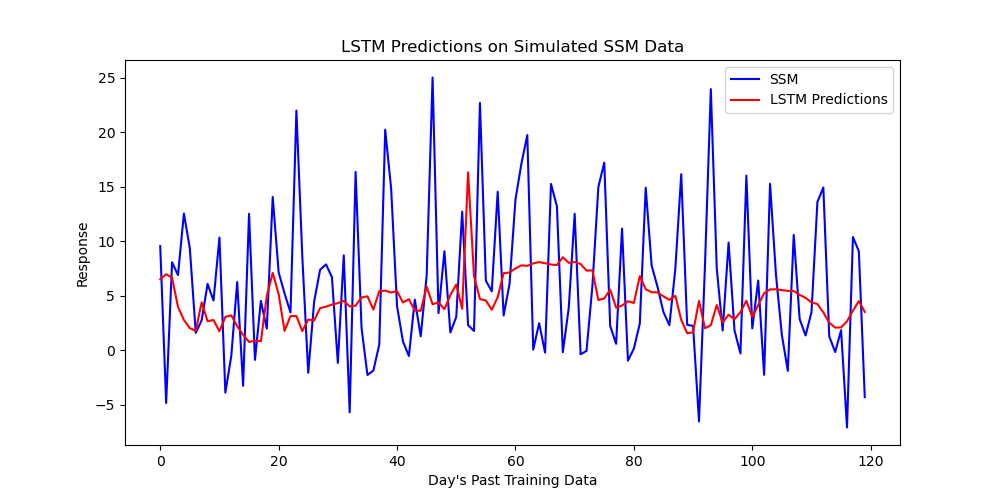
\includegraphics[width=0.5\linewidth]{"Figures/Model Diagnostics/SSM_model_1.png"}}
    \subfloat[4,000]{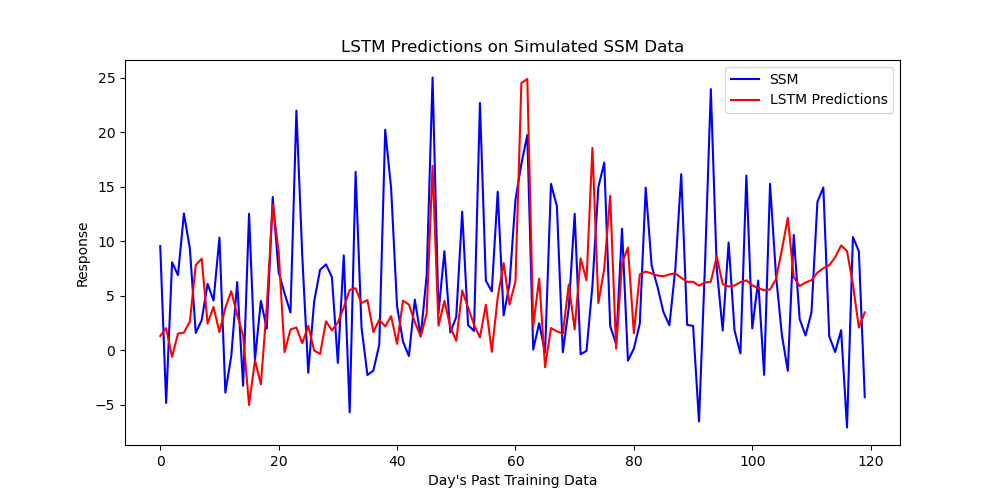
\includegraphics[width=0.5\linewidth]{"Figures/Model Diagnostics/SSM_model_3.png"}}\\
    \subfloat[6,000]{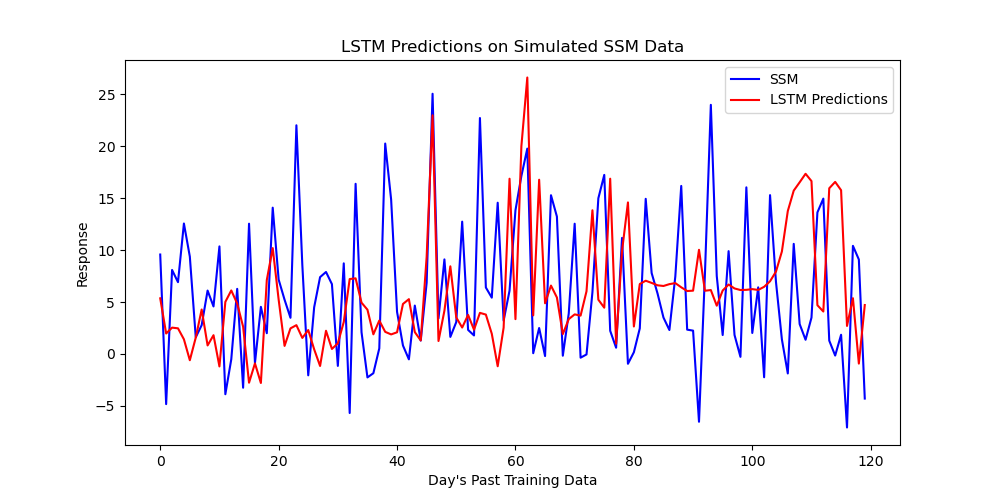
\includegraphics[width = 0.5\linewidth]{"Figures/Model Diagnostics/SSM_model_5.png"}}
    \subfloat[8,000]{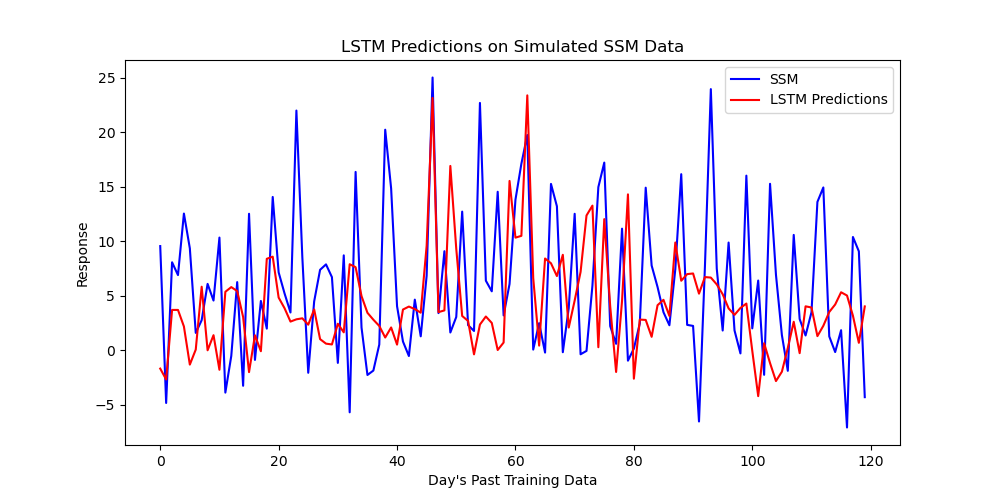
\includegraphics[width = 0.5\linewidth]{"Figures/Model Diagnostics/SSM_model_7.png"}}\\
    \subfloat[10,000]{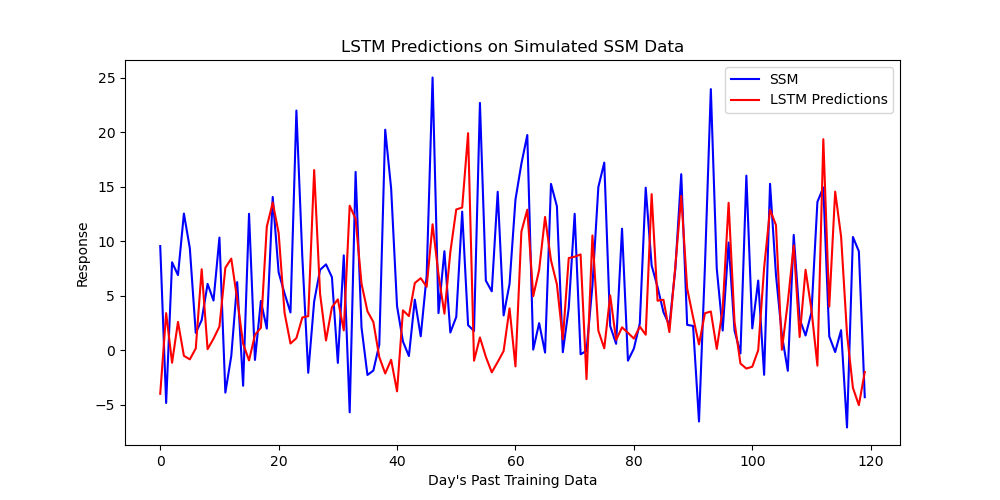
\includegraphics[width=0.5\linewidth]{"Figures/Model Diagnostics/SSM_model_9.png"}}
    \subfloat[12,000]{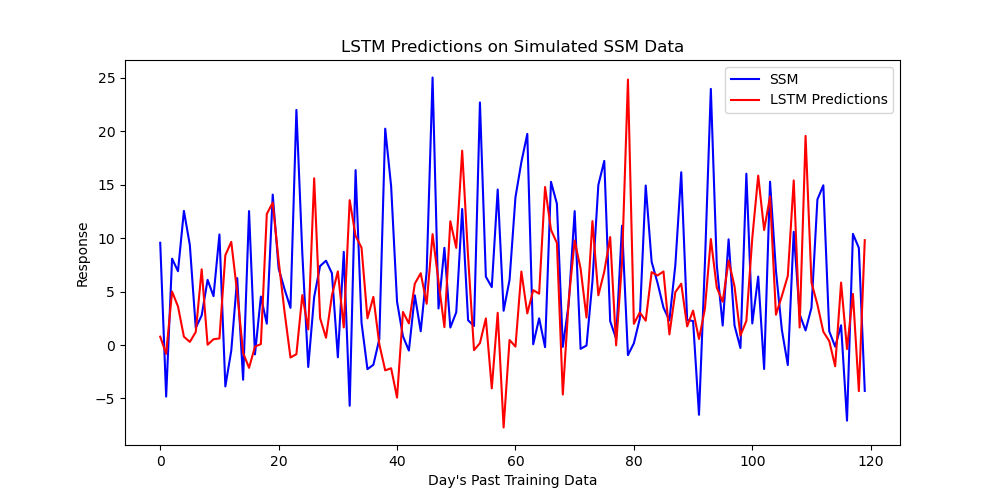
\includegraphics[width=0.5\linewidth]{"Figures/Model Diagnostics/SSM_model_11.png"}}
    \caption{A plot showing the LSTM predictions during the training process on the SSM simulated data.}
    \label{fig:SSMTraining}
\end{figure}
\FloatBarrier
